\documentclass[../candidatura.tex]{subfiles}
\graphicspath{{\subfix{../imagenes/}}}
\begin{document}

\section{Investigación propuesta}

% en borradores iniciales, la extensión sugerida era de diez páginas

\subsection{Presentación del proyecto}

% Marco general  de la investigación
% Pregunta de investigación o hipótesis
% Objetivos
% Metodología
% Resultados esperados

% con esto, propongo los siguientes párrafos

% intro
En el siglo XXI la construcción de sintetizadores sonoros ha experimentado una fuerte expansión industrial y artesanal impulsada por software y hardware con licencias permisivas, adopción de herramientas de fabricación digital paramétrica y abaratamiento de costos de distribución de materias primas mediante internet. La gran barrera que aún existe es que este conocimiento continúa distribuido de manera fragmentada, especializada y concentrada en determinados polos hegemónicos entrelazados en lo geográfico, lingüístico y productivo. Esta investigación doctoral propone la popusintesíntesis como un marco conceptual y práctico para comprender y ampliar la producción popular de sintetizadores, entendiendo dicha práctica no sólo como el diseño de sintetizadores, sino también como la creación de las infraestructuras técnicas, pedagógicas, culturales y materiales que hacen posible su puesta en escena. Siguiendo a Sara Ahmed, para quien la orientación vuelve familiar lo extraño a fuerza de habitarlo, y la desorientación ocurre cuando esa operación falla \footcite{ahmed_fenomenologia_2024}, la popusintesíntesis propone desorientar la relación habitual con los sintetizadores como cajas negras de consumo, para reorientarla hacia su fabricación, reparación y modificación.

% Marco general  de la investigación
La investigación se sitúa desde Chile en el siglo XXI como un contexto caracterizado por un alto consumo de tecnologías electrónicas y computacionales, pero una baja producción local de estas infraestructuras. Desde este lugar de enunciación se exploran estrategias abiertas, reparables y permisivas que permitan crear y robustecer capacidades locales de diseño y fabricación de sintetizadores.

% Pregunta de investigación o hipótesis

A partir de este contexto, la investigación pregunta cómo la popusintesíntesis, entendida como una práctica artística pública, abierta, reparable, legible, asequible y artesanal, genera estrategias de diseño y fabricación alternativas a las industrias, que permitan popularizar la producción de ruidos y conocimientos técnicos, y favorecer la autonomía tecnológica en polos tradicionalmente considerados de baja productividad electrónica y computacional.

% Objetivos

Esta tesis desarrolla simultáneamente un marco conceptual para la popusintesíntesis y una serie de artefactos electrónicos y computacionales que materializan en máquinas estas ideas. Los objetivos consideran la construcción de un glosario conceptual, el desarrollo de infraestructura electrónica y computacional, y la sistematización de estrategias de documentación y enseñanza que permitan reproducir y adaptar estos conocimientos a distintos contextos productivos y culturales.

% Metodología

Metodológicamente, la investigación combina revisión bibliográfica, análisis de referentes artísticos e industriales, prototipado iterativo de dispositivos electrónicos y software, documentación abierta y validación mediante docencia, uso artístico y publicación de los resultados bajo licencias abiertas. El proceso investigativo entiende el diseño, la fabricación y la documentación como actividades inseparables para la creación de herramientas artísticas, en particular sintetizadores sonoros.

% Resultados esperados

Se espera que esta investigación contribuya con un nuevo marco conceptual para comprender y fomentar la síntesis popular de sintetizadores, así como con un conjunto de módulos electrónicos, bibliotecas computacionales, manuales y estrategias metodológicas que faciliten la creación de nuevos sintetizadores. En conjunto, estos resultados buscan disminuir barreras de acceso al conocimiento técnico, fortalecer prácticas locales de fabricación y ampliar las posibilidades de investigación artística en torno al sonido y el ruido.

\subsection{Lugar de enunciación}

Esta práctica artística y académica es una mezcla de confluencias y contradicciones, donde se aspira a no ser aspiracional, a popularizar la producción de ruido para fines artísticos, a promover el goce del sonido desatado en distintas manifestaciones, a desencadenar modulaciones no hegemónicas \footcite{mendivil_contra_2023}, a valorar la infraestructura material y cultural que permite sonar y escuchar.

Como lugar de enunciación desde donde se realiza esta investigación, se propone Chile en el año 2026 como un polo de alto consumo electrónico y computacional, y al mismo tiempo un polo de baja producción electrónica y computacional, donde muy pocas personas han logrado acceder a la producción de sintetizadores, y muchas de ellas han emigrado a otras latitudes donde desarrollar su práctica.

Este lugar de enunciación también incluye al computador como taller y la internet como fabricante, donde se han abaratado los costos de diseño de electrónica y computación, permitiendo que en el mundo existan talleres unipersonales de diseño de sintetizadores, con fabricación distribuida en distintos polos de producción como China y Estados Unidos.

La capa autoral de este lugar de enunciación corresponde a mi propia práctica como persona que emite ruido, que consume sintetizadores, que produce software, que diseña y fabrica electrónica, que enseña en academia sobre estas prácticas, y que tiene reparos críticos: los sintetizadores que he usado en mi última década son instrumentos profesionales que me inspiran, pero su alto costo monetario me impide compartirlos ampliamente con más artistas y estudiantes. Después de casi una década viviendo fuera de Santiago formándome en distintas disciplinas, he vuelto a fabricar electrónica, he entrenado a estudiantes que ahora son mis colaboradores, se han abierto nuevos espacios en academia que me acogen y me nutren como artista y como investigadora, y he formado alianzas con personas, instituciones y empresas que me permiten materializar el sueño de la popusintesíntesis, de quitar barreras a la producción de sintetizadores, de que tal como existen las guitarras arrumbadas en las esquinas de muchas casas, existan también sintetizadores.

Este lugar de enunciación, tal como una PCB, tiene muchas capas de conexiones, sustratos, aislantes, cortocircuitos, islas, vías y tierras, que en su conjunto permiten esta investigación. También esta investigación es un homenaje, tributo y por sobre todo un puente de conexión a otras prácticas artísticas, tal como los cables que conectan distintos módulos en un sintetizador ruidista.

\subsection{Motivaciones}

Las motivaciones que llevan a la realización de esta tesis doctoral son múltiples, entre las que destacan las siguientes.

\subsubsection{Transdisciplina popular artesanal}

La formación académica necesaria para la construcción de sintetizadores generalmente necesita de un tránsito entre muchas disciplinas, incluyendo física, ingeniería eléctrica, matemática, carpintería, ciencias de la computación, diseño industrial, bellas artes, entre otras. Esta tesis emerge como una forma de promover que la síntesis de sintetizadores sea una práctica popular transdisciplinar y artesanal \footcite{collins_handmade_2020}, no anecdótica ni alimentada por esfuerzos individuales, ni tampoco necesariamente realizada en polos tradicionales productivos de electrónica y computación, como lo son China y Estados Unidos.

\subsubsection{Materia por sobre cultura}

Esta investigación es realizada para poder establecer un diálogo con la materia, que ocurran sonidos a partir de componentes que dependen de su fisicalidad, pero no de nociones culturales preconcebidas dominantes en la música como armonía, ritmos, o afinaciones. Una motivación fuerte es no promover tradiciones hegemónicas en la producción sonora o de instrumentos, sino que emerjan nuevas formas donde las barreras sean físicas y no mentales ni estéticas.

\subsection{Marco teórico / definiciones conceptuales}
\label{subsec:marco-teorico}


En industria y en español existe muchas veces una amalgama entre conceptos como sintetizadores y teclados, pero esta tesis se concentra en otros tipos de interfaces \footcite{bjorn_push_2021} y gestualidades para la síntesis sonora.

En la industria contemporánea de la síntesis también existe mucho énfasis en música, lo que está divorciado del origen artístico e investigativo de muchas personas pioneras del siglo XX que expandieron el campo del arte sonoro y sentaron las bases cartográficas, conceptuales, electrónicas y computacionales \footcite{roads_computer_1996} que permiten la emergencia de un amplio abanico de sintetizadores actuales y futuros.

El mismo concepto de industria está también en tensión con gran parte de las referentes citadas en esta investigación, quienes difuminan las barreras entre luthería, composición e interpretación, muchas veces dedicándose a todas ellas al mismo tiempo.

La síntesis emerge como poética en el sentido de crear. La sintesíntesis es a los skateparks, como la síntesis es al skate. La sintesíntesis tiene que ver con crear la infraestructura para que otras personas puedan hacer sus piruetas encima del pavimento.

La palabra popular añade una pizca de tensión, donde se pide amplitud de mente para incorporar lo electrónico y computacional a las prácticas populares. El sueño entonces explícito es que los productos de esta tesis, los sintetizadores sonoros, sean tan populares que puedan compartirse tanto en ferias como en tiendas de productos típicos como Artesanías de Chile.

Una de las acepciones de lo popular que asume esta tesis es la de la educación popular propuesta por el filósofo brasileño Paulo Freire. Distingue entre una teoría de la acción antidialógica, caracterizada por la conquista, la división para oprimir, la manipulación y la invasión cultural, y una teoría de la acción dialógica, caracterizada por la colaboración, la unión, la organización y la síntesis cultural \footcite{freire_pedagogia_1970}. Es una coincidencia afortunada que la síntesis aparezca en Freire como lo opuesto a la invasión cultural: mientras la invasión impone la visión del mundo de quien llega desde fuera, la síntesis cultural se construye en conjunto, de forma popular.

Otra acepción de lo popular es la de lo masivo y asequible. Tatsuya Takahashi, diseñador de sintetizadores \footcite{james_takahashi_2017}, en su primera era trabajando en la empresa japonesa KORG entre 2010 y 2017 como ingeniero jefe de sintetizadores análogos, publicó un post en Facebook donde celebraba que los Korg volca fueran el primer sintetizador de infancias aprendiendo música, y que eso resonaba con el nombre volca, en alusión a la palabra alemana Volk, y a otras marcas como Volkswagen, el auto del pueblo. Así, Tatsuya propone a los Korg volca como sintetizadores de la gente, populares \footcite{synthtopia_takahashi_2017}. En su visión, lo popular no termina en la compra del instrumento: sus diseños incluyen guiños a quienes quieran abrirlos y modificarlos, como la publicación de los esquemáticos del Korg monotron y las serigrafías en sus placas de circuito impreso que invitan a soldar nuevas conexiones \footcite{korg_monotron_sinfecha}. En conexión paralela, el autor peruano Manuel Scorza fundó la empresa Populibros Peruanos, que estuvo operativa entre 1963 y 1965, publicando más de 60 títulos y vendiendo casi un millón de ejemplares a bajo costo en su país natal \footcite{aguirre_populibros_2017}. Esta tesis asume de esta acepción la búsqueda de costos bajos y componentes sin escasez mediante la producción masiva e industrial, pero se distancia de su forma corporativa: un instrumento asequible que sigue siendo una caja negra no es suficientemente popular.

Una tercera acepción es la de lo popular como público y abierto, en el sentido de los movimientos y legalidades detrás del software y el hardware de fuente abierta. Organizaciones como la Open Source Hardware Association y CERN han desarrollado definiciones y licencias que permiten compartir esquemáticos, códigos y técnicas de fabricación \footcites{oshwa_about_sinfecha}{cern_ohl_sinfecha}. Esta tesis asume que la apertura legal es necesaria pero insuficiente: un circuito abierto pero ilegible, sin documentación o solamente en inglés, sigue siendo nicho. Por eso se proponen la legibilidad y la consecuente reparabilidad como condiciones de lo popular.

% criterios operativos de lo popular
A partir de esta constelación de acepciones, en esta tesis se considera que un sintetizador es popular cuando cumple con los siguientes criterios: su costo de materiales es bajo, sus componentes son asequibles y sin escasez; sus esquemáticos, códigos y documentación se publican con licencias permisivas; su documentación está disponible en español; puede ser reparado, clonado y modificado por otras personas; y su diseño invita al ruido y a la experimentación, no a la imposición de reglas ni de consumo pasivo.

A nivel de crítica sobre los objetos de estudio, se referenciarán los estudios de la última década de Yuk Hui \footcites{hui_existence_2016}{hui_arte_2025}, donde se proponen metodologías filosóficas de enfrentarse a objetos digitales, que a su vez son el sustrato que permite la construcción y programación de sintetizadores sonoros computacionales.

\subsection{Problema / objeto de estudio / corpus}

El objeto de estudio es la síntesis popular de sintetizadores, encarnada en individuos y empresas que se dedican al diseño, implementación y fabricación de sintetizadores sonoros, los libros y materiales educativos que permiten esta práctica transdisciplinar, las instituciones donde se imparten cursos y residencias en torno a la síntesis de sintetizadores, y de forma aún más amplia a la gente desarrolladora de software y hardware y bibliotecas que hace posible la sintesíntesis popular en distintos lenguajes y paradigmas.

\subsection{Criterios de selección del corpus}

Los criterios de selección del corpus responden a las ideas fuerza de esta investigación: se seleccionan fuentes, obras y prácticas que hacen visible el conocimiento técnico en lugar de ocultarlo, que lo comparten mediante licencias abiertas o la docencia, que lo sitúan en contextos productivos no hegemónicos, y que entienden la fabricación de instrumentos como práctica artística.

\subsubsection{Selección de corpus bibliográficos}

Dado el abismo de información técnica que esta tesis incluye, es necesario contrapesar con filosofía sobre electrónica, computación, ruido, entre otras.

En este corpus se priorizan libros de la última década que sistematizan prácticas artísticas y pedagógicas, tanto en electrónica \footcite{pearson_electronic_2024} como en computación \footcite{erwig_erase_2025}. También se incluyen libros históricos del siglo XX sobre distintos sintetizadores sonoros \footcite{pinch_analog_2002} y artefactos electrónicos y computacionales asociados.

Los libros técnicos y pedagógicos aportan el vocabulario y las estrategias de enseñanza que esta tesis busca traducir y adaptar al español, mientras la filosofía aporta herramientas para leer críticamente estos objetos técnicos.

\subsubsection{Selección de corpus artísticos}

En el corpus estudiado se incorporan las obras de artistas que son relevantes y por sobre todo inspiradoras en la travesía de la popusintesíntesis.

Se escogen las voces generosas que realizan docencia, que comparten sus procesos, que realizan conciertos, actividades de difusión, que celebran la escena de personas prospectando y fabricando sintetizadores, o que realizan obras de formas populares y abiertas.

Estas obras aportan modelos de cómo una práctica artística puede abrir su taller a otras personas.

\subsubsection{Selección de corpus productivos}

Se priorizan distintas técnicas amigables con el medio ambiente, desde certificaciones RoHS, hasta legibilidad y reparabilidad de sintetizadores de uso flexible.

Se describen prácticas paramétricas como las realizadas por Peter Blasser, quien de forma rumiante a lo largo de los años ha publicado circuitos, luego con ellos ha realizado instalaciones artísticas y productos artesanales, y con los años estos han mutado a productos industriales hechos en fábricas por equipos de múltiples personas.

En el corpus se incluyen también los sintetizadores lanzados por empresas como BASTL Instruments, Ciat-Lonbarde, Critter and Guitari, que han operado bajo principios de software y hardware abierto, que apuestan por la electrónica y la computación como una forma de compartir y de potenciar a artistas a que modifiquen sus propios instrumentos.

Estas empresas y prácticas demuestran que es viable producir y comercializar sintetizadores abiertos, y aportan estrategias concretas de fabricación, costos y licencias.

\subsubsection{Selección de corpus de obras personales}

En obras personales incluyo obras y series de obras artísticas realizadas a través de los últimos 15 años que tributan a la popusintesíntesis.

Algunas de mis obras son los cursos que dicto en pregrado, donde enseño formas de leer y de entender electrónica y computación, además de mentorear a estudiantes que también se dedican a la docencia como ayudantes, y que están realizando proyectos de investigación en pregrado.

Otra parte de mi obra personal tiene que ver con herramientas que he desarrollado para mi taller, que son paramétricas, abiertas y que permiten la difusión de las herramientas que trabajo.

Otra gran obra o metaobra es la empresa piruetas SpA, un estudio de arte electrónico chileno, con el cual tomo comisiones de proyectos para recaudar dinero y aplicar mi investigación, donde compro materiales con factura, aprendo a importar, a tener un inventario y a comercializar sintetizadores.

Estas obras son parte del corpus porque son el lugar donde se ponen a prueba los criterios de evaluación propuestos en la metodología de esta tesis.

\subsection{Referencias críticas sobre objeto de estudio / estado del arte}

La popusintesíntesis es un fenómeno transdisciplinar que ha sido estudiado desde distintas aristas disciplinares, incluyendo: la historia de las invenciones electrónicas usadas para síntesis sonora, los avances industriales productivos en tecnologías para fabricación de máquinas electrónicas y computacionales, las estéticas punk y del hazlo-tú-misma y su impacto en microempresas y en lo doméstico, las propuestas de permacomputación, las discusiones y licencias de software y hardware libre y de fuente abierta, además de las prácticas cacharreras latinoamericanas.

Este estado del arte es una constelación de referencias que prueba la existencia de un campo amplio y fragmentado: existen conocimientos desperdigados sobre cómo realizar popusintesíntesis, pero está repartido entre distintas disciplinas, idiomas, polos productivos, y presupone en muchos casos formaciones altamente técnicas. Aquí emerge la oportunidad y el valor de proponer la popusintesíntesis como un campo de estudio en esta tesis doctoral.

\subsubsection{Historia de la industria de sintetizadores}

% 1. historia e industria del sintetizador
Los estudios sobre la historia del sintetizador han documentado su emergencia como artefacto industrial y cultural en el siglo XX \footcite{pinch_analog_2002}, mostrando cómo las decisiones de diseño, comercialización y uso co-construyeron el sintetizador Moog. Sin embargo, estos estudios se concentran en polos productivos de Estados Unidos, Europa y Japón, y tratan la fabricación como asunto de empresas más que como práctica popular.

\subsubsection{Electrónica artesanal y hazlo-tú-misma}

Una segunda línea sistematiza la construcción de instrumentos electrónicos fuera de la industria, como manuales de electrónica artesanal \footcite{collins_handmade_2020} y las publicaciones de la conferencia internacional NIME (New Interfaces for Musical Expression) sobre instrumentos abiertos y hazlo-tú-misma \footcite{nime_sinfecha}. Estas aproximaciones sortean barreras técnicas, pero están mayoritariamente en inglés, y suelen centrarse en un instrumento o técnica puntual más que en la infraestructura que permite su reproducción, y están escritas para un público especializado y con conocimientos previos.

\subsubsection{Software y hardware libres, abiertos y públicos}

El movimiento hacker, de software libre, de fuente abierta y sus distintas facciones \footcite{tozzi_history_2017} han tenido que lidiar con las legalidades y licencias de las herramientas que producen, de sus implicancias sociales y comerciales, de patentes, copyright, derechos y créditos.

En paralelo existe el movimiento de hardware libre, donde el mayor exponente actual es la Open Source Hardware Association, quienes permiten a una comunidad mundial compartir sus trabajos de formas libres, que resguarden una mezcla de la propiedad intelectual, de compartir diseños, de créditos.

Los sintetizadores tienden a tener ciertas libertades y ciertas opacidades. KORG ha lanzado instrumentos como drumlogue con una SDK abierta y gratuita, Critter and Guitari permite a personas modificar el software y firmware de su instrumento Organelle que corre Pure Data, permitiendo que una comunidad de artistas comparta código de osciladores, efectos y estrategias de composición y performance.

Que el código sea abierto no necesariamente lo hace popular, se requiere que el código sea legible, esté documentado, que tenga licencias permisivas que permitan compartirlo.

Las bicicletas son una gran inspiración de la popusintesíntesis y la encarnan: no existen patentes que restrinjan a fabricantes lanzar nuevas bicicletas, tampoco existen barreras en el uso de las bicicletas que restrinjan su uso, que no puedan transitar ciertos caminos. Tampoco son instrumentos utilitarios que solamente cumplan con el fin de transportarte de un lugar a otro de forma eficiente. Las bicicletas son por sobre todo experiencia, piruetas, un instrumento de arte popular.

\subsubsection{Reparabilidad, sustentabilidad y permacomputación}

Pensar la electrónica desde la reparabilidad y la sustentabilidad implica también revisar las nociones de energía y trabajo que la electrónica hereda de la termodinámica y de la industria de los combustibles fósiles \footcite{daggett_birth_2019}.

Los sintetizadores son instrumentos con muchas capas, desde la interfaz, la carcasa, la circuitería, por lo que su reciclabilidad es difícil. Una forma de combatir la obsolescencia es diseñar sintetizadores con componentes que no colapsen en el corto plazo. Un ejemplo es el artista Peter Blasser, quien evita los capacitores electrolíticos ya que normalmente expiran en un plazo de entre 20 y 40 años\footcite{tagi_blasser_2023}.

El dúo de artistas Hundred Rabbits tiene una práctica multimedia, donde postulan que las herramientas que usan y publican son reparables sin intervención de elles directamente, gracias a la documentación que las acompaña\footcite{hundredrabbits_about_sinfecha}. Su obra promueve la permacomputación\footcite{hundredrabbits_permacomputing_sinfecha}, y en pos de ella, han creado Uxn, una máquina virtual de bajo consumo, y han creado software de uso para su taller que corre sobre ella, incluyendo editores de texto y herramientas para hacer música.

Para poder asegurar el carácter popular de las obras creadas en pos de la sintesíntesis, se incluye en este estado del arte el trabajo realizado por organizaciones como Creative Commons, MIT, Open Source Hardware Association, y CERN para crear licencias, para dar tribuna y gremialidad a la creación de hardware público, permitiendo el dar un marco legal de compartir esquemáticos, documentación y técnicas de fabricación de hardware y sintetizadores.

\subsubsection{Prácticas latinoamericanas y no hegemónicas}

El desarrollo de sintetizadores ha proliferado en los polos tradicionales de desarrollo de electrónica y computación, destacando Estados Unidos, Japón, Alemania, Inglaterra, Francia, entre otros.

Por otro lado, Latinoamérica y Chile se han mantenido como lugares distantes a estos polos de producción, ocupando un rol de consumidor más que de productor de sintetizadores sonoros, o donde los esfuerzos en la producción han sido llevados a cabo por esfuerzos personales o pequeñas colectividades.

Dentro de ese panorama industrial, emergen esfuerzos individuales en lugares físicos y metodológicos no hegemónicos. Desde la década de los 2000 han surgido empresas abocadas al desarrollo de instrumentos como BASTL (República Checa), Oficina de Sonido (Chile, México), Sonic Liberation Devices (Estados Unidos), quienes gracias al desplome de los costos de producción de electrónica han podido diseñar desde talleres en lugares no hegemónicos, con equipos pequeños, fabricar con herramientas locales y mundiales, y con eso influir en sus escenas locales y mundiales.

\subsection{Referentes artísticos y contexto en que se sitúa la práctica artística}

Los grandes referentes artísticos sobre los que se sitúa esta práctica artística incluyen, entre otras, a las siguientes gigantes de la sintesíntesis.

\subsubsection{Ciat-Lonbarde}

Peter Blasser es un artista que ha desarrollado varias líneas de sintetizadores en los últimos 20 años, entre ellos los samplers, órganos y máquinas de ritmo de Ciat-Lonbarde, los instrumentos programables de Shbobo como Shnth y Shtar, y su más reciente familia de sintetizadores Cafe Quantum \footcite{patchpoint_cafequantum_2025}.

\begin{figure}[!htbp]
    \centering
    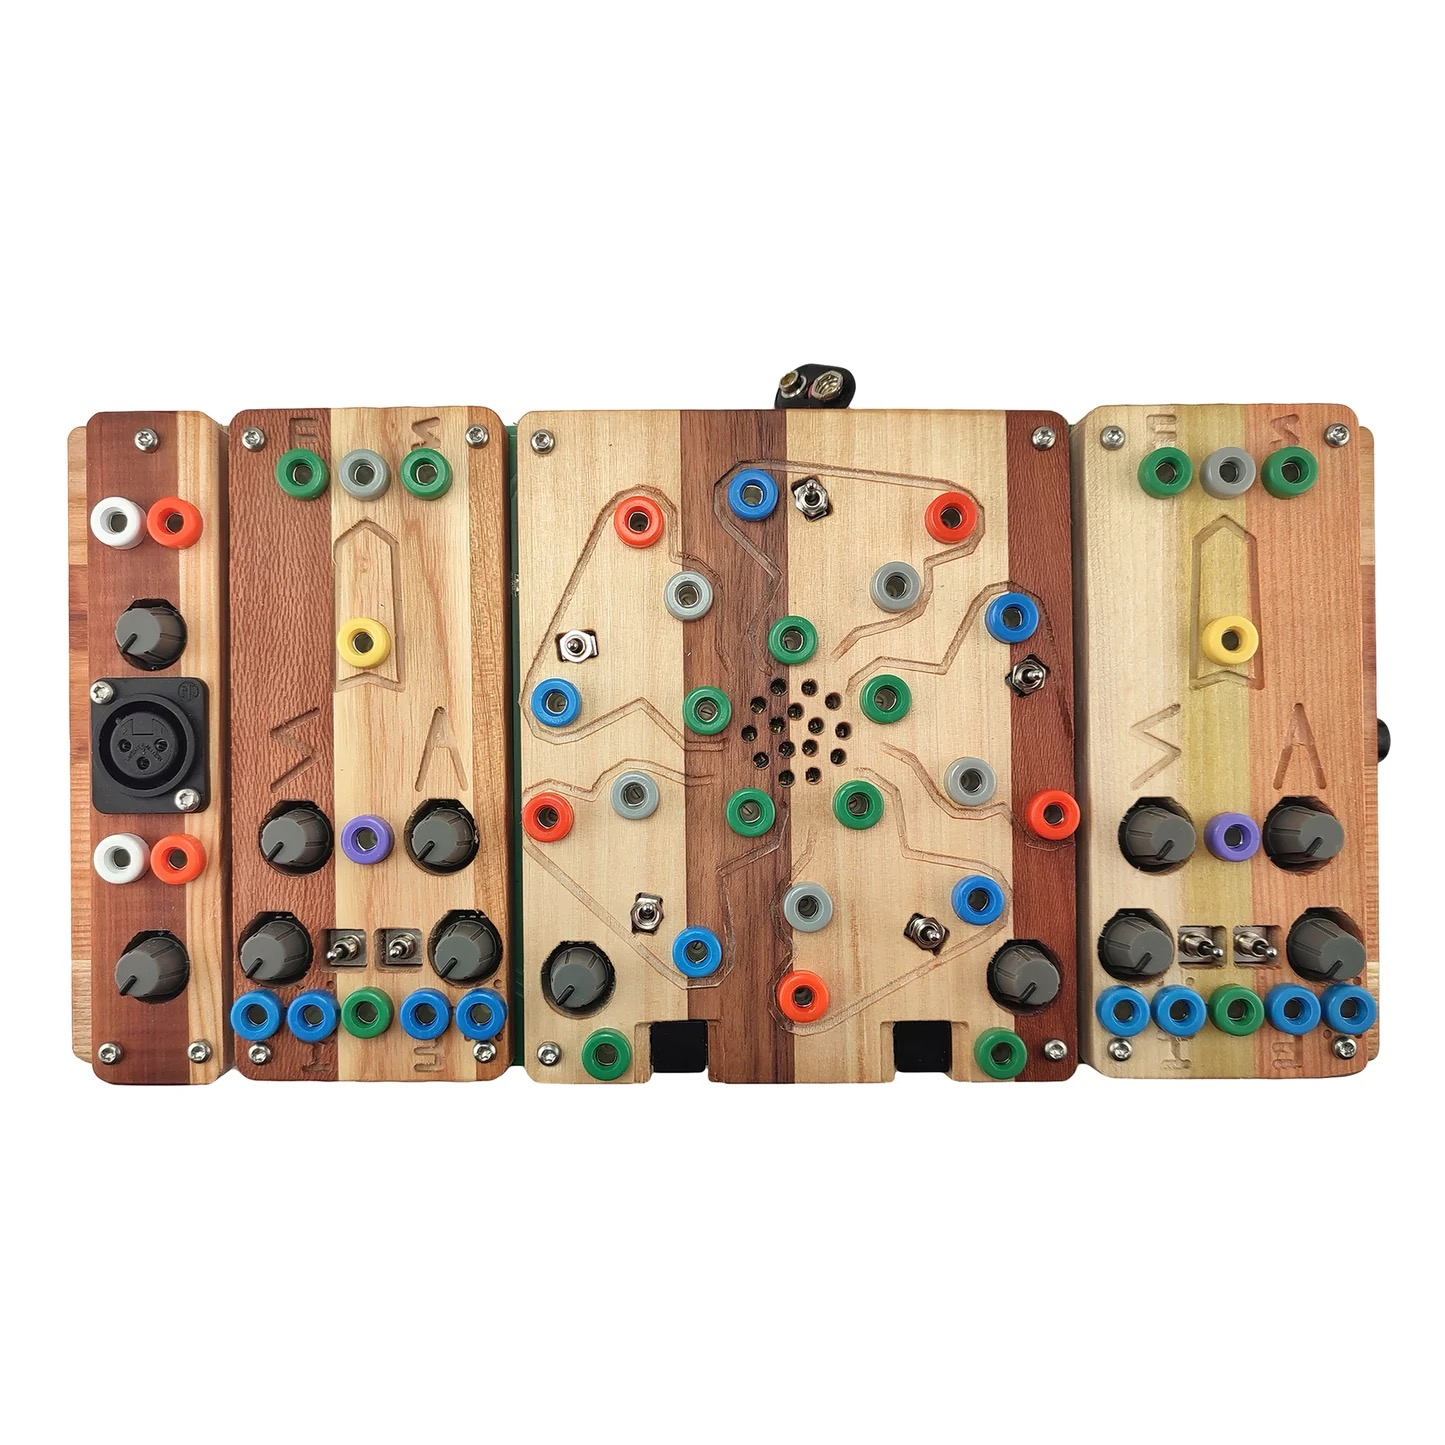
\includegraphics[width=0.6\textwidth,trim={0 405bp 0 405bp},clip]{./imagenes/referencias/ciat-lonbarde-cocoquantus.jpg}
    \caption[Cocoquantus 2, Ciat-Lonbarde]{Instrumento Cocoquantus 2 de Ciat-Lonbarde. Fuente: \parencite{patchpoint_cocoquantus_sinfecha}.}
    \label{fig:ciat-lonbarde-cocoquantus}
\end{figure}

Ciat-Lonbarde propone sintetizadores modulares sin pantallas, algunos programables, con metáforas para explicar la producción de sus sonidos, con distintos paradigmas ruidistas de codificación de colores en sus nodos de conexión, y con la propuesta de no cuantizar ni ritmos ni frecuencias en modos hegemónicos ni clasicistas.

\subsubsection{Clacktronics}

La empresa inglesa Clacktronics lanzó un libro con paneles prepicados para romperlos y luego poblarlos con componentes electrónicos, soldarlos y convertirlos en un sintetizador modular en formato Eurorack, incluyendo la carcasa dentro del libro. La licencia es permisiva, el software y hardware es de fuente abierta y permite aprender de este sintetizador y adaptarlo a nuevas creaciones.

\begin{figure}[!htbp]
    \centering
    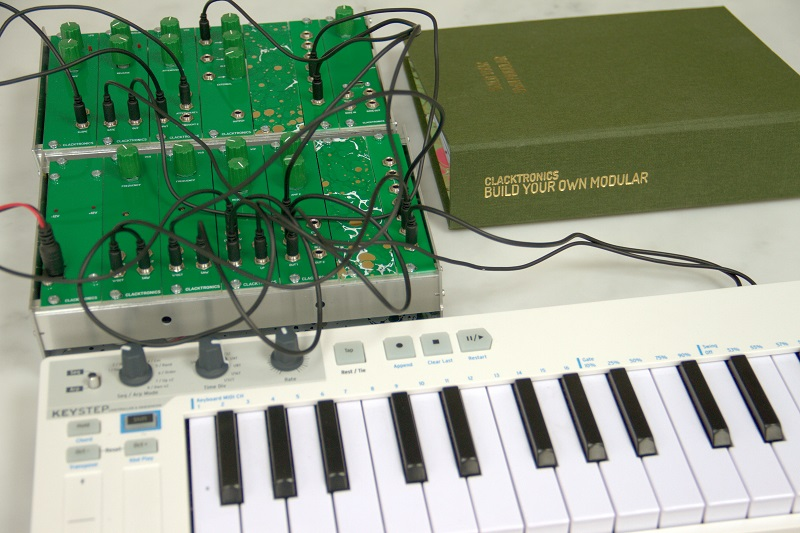
\includegraphics[width=0.6\textwidth,height=5cm,keepaspectratio]{./imagenes/referencias/clacktronics-build-your-own-modular.jpg}
    \caption[Build Your Own Modular, Clacktronics]{Build Your Own Modular de Clacktronics. Fuente: \parencite{clacktronics_buildyourownmodular_sinfecha}.}
    \label{fig:clacktronics-build-your-own-modular}
\end{figure}

\subsubsection{Corazón de Robota}

La artista Constanza Piña, con su alias Corazón de Robota, ha desarrollado una práctica de creación de sintetizadores, material de enseñanza DIY, talleres e infraestructura para enseñar y promover la creación de sintetizadores a partir de circuitos integrados y distintos sensores. Sus performances y su práctica artística están hechos con series de instrumentos diseñados y fabricados por ella, a partir de técnicas modulares, de soldadura punto a punto, y de tradición ruidista.

\begin{figure}[!htbp]
    \centering
    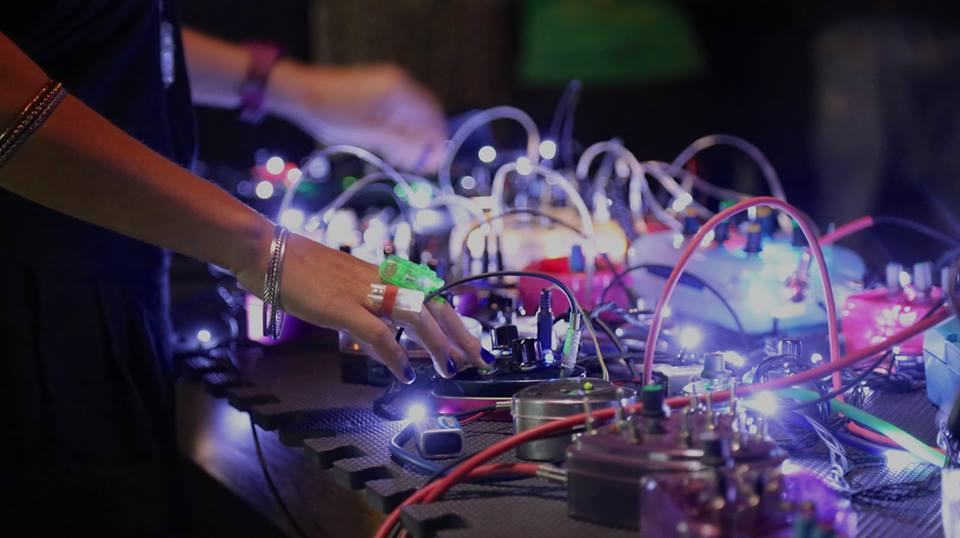
\includegraphics[width=0.6\textwidth,height=5cm,keepaspectratio]{./imagenes/referencias/corazon-de-robota.jpg}
    \caption[Corazón de Robota, Constanza Piña]{Corazón de Robota de Constanza Piña. Fuente: \parencite{constanzapina_corazonderobota_sinfecha}.}
    \label{fig:constanza-pina-corazon-de-robota}
\end{figure}

\subsubsection{Critter and Guitari}

En esta última década esta empresa ha lanzado varias iteraciones de 2 productos programables: Organelle, un sintetizador de sonido programable en el lenguaje Pure Data, y Eyesy, un sintetizador de video programable en el lenguaje Python. Existen comunidades de desarrolladores y artistas que comparten instrumentos y código con estas plataformas.

\begin{figure}[!htbp]
    \centering
    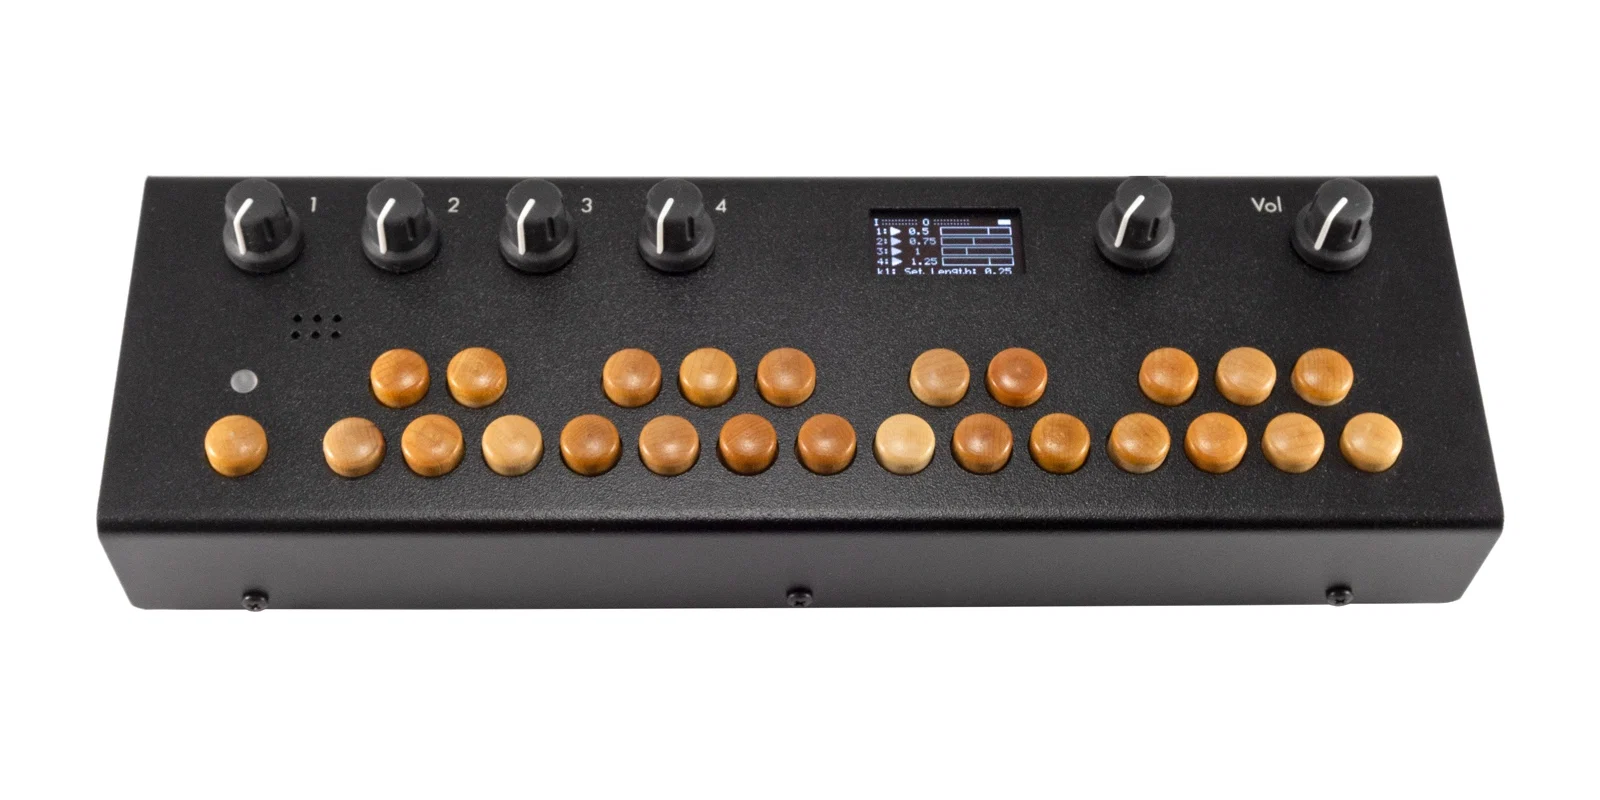
\includegraphics[width=0.6\textwidth,height=5cm,keepaspectratio]{./imagenes/referencias/critter-and-guitari-organelle.jpg}
    \caption[Organelle, Critter and Guitari]{Organelle de Critter and Guitari. Fuente: \parencite{critterandguitari_organelle_sinfecha}.}
    \label{fig:critter-and-guitari-organelle}
\end{figure}

\subsubsection{Flower Electronics}

La empresa estadounidense Flower Electronics estuvo activa entre 2006 y 2013 produciendo distintos sintetizadores modulares, destacando Little Boy Blue y Jealous Heart. Al igual que los instrumentos de Ciat-Lonbarde, heredan la tradición de Buchla de usar cables banana para realizar las conexiones entre distintos nodos del instrumento. Destaco a esta empresa como referente al incluir en sus manuales instrucciones de cuidado del instrumento, además de promoverse como una empresa de instrumentos hechos a mano, y a pesar de declararse como musical, hace énfasis en ruidismo.

\begin{figure}[!htbp]
    \centering
    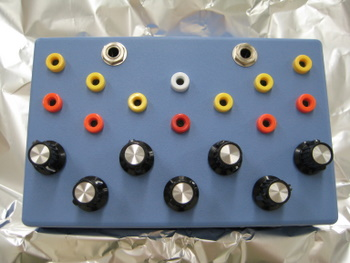
\includegraphics[width=0.6\textwidth,height=5cm,keepaspectratio]{./imagenes/referencias/flower-electronics-little-boy-blue.jpg}
    \caption[Little Boy Blue, Flower Electronics]{Little Boy Blue de Flower Electronics. Fuente: \parencite{flowerelectronics_littleboyblue_sinfecha}.}
    \label{fig:flower-electronics-little-boy-blue}
\end{figure}


\subsubsection{KORG}

La empresa japonesa KORG históricamente ha lanzado sintetizadores con distintos grados de permisos para usuarios. Para este trabajo se destaca el trabajo de la última década, que incluye lanzamientos de una línea de sintetizadores programables con su propia SDK, incluyendo a minilogue xd, drumlogue, prologue y nts-1 mk1 y mk2.

\begin{figure}[!htbp]
    \centering
    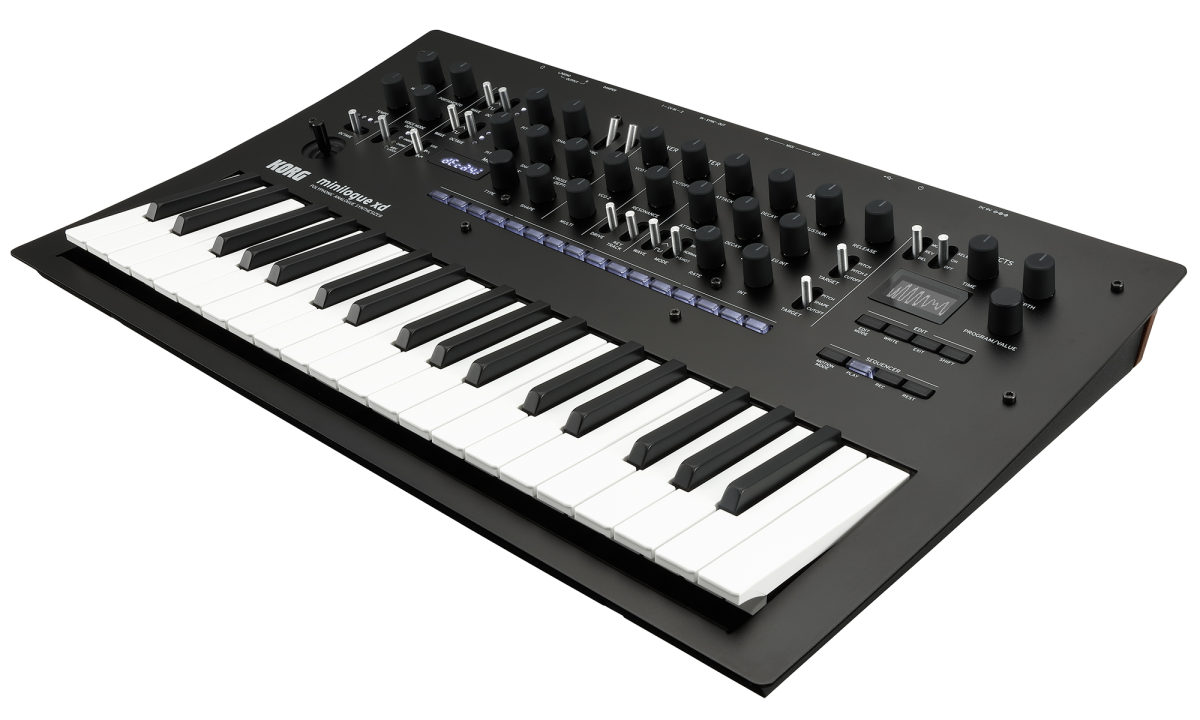
\includegraphics[width=0.6\textwidth,height=5cm,keepaspectratio]{./imagenes/referencias/korg-minilogue-xd.png}
    \caption[minilogue xd, KORG]{minilogue xd de KORG. Fuente: \parencite{korg_miniloguexd_sinfecha}.}
    \label{fig:korg-minilogue-xd}
\end{figure}

\subsubsection{Oficina de Sonido}

La empresa de Daniel Llermaly ha lanzado varios sintetizadores, entre ellos un sistema modular con el estándar Eurorack llamado My First Modular, y un instrumento electrónico Hanan Cumbia, inspirado en Bleep Drum de Bleep Labs.

\begin{figure}[!htbp]
    \centering
    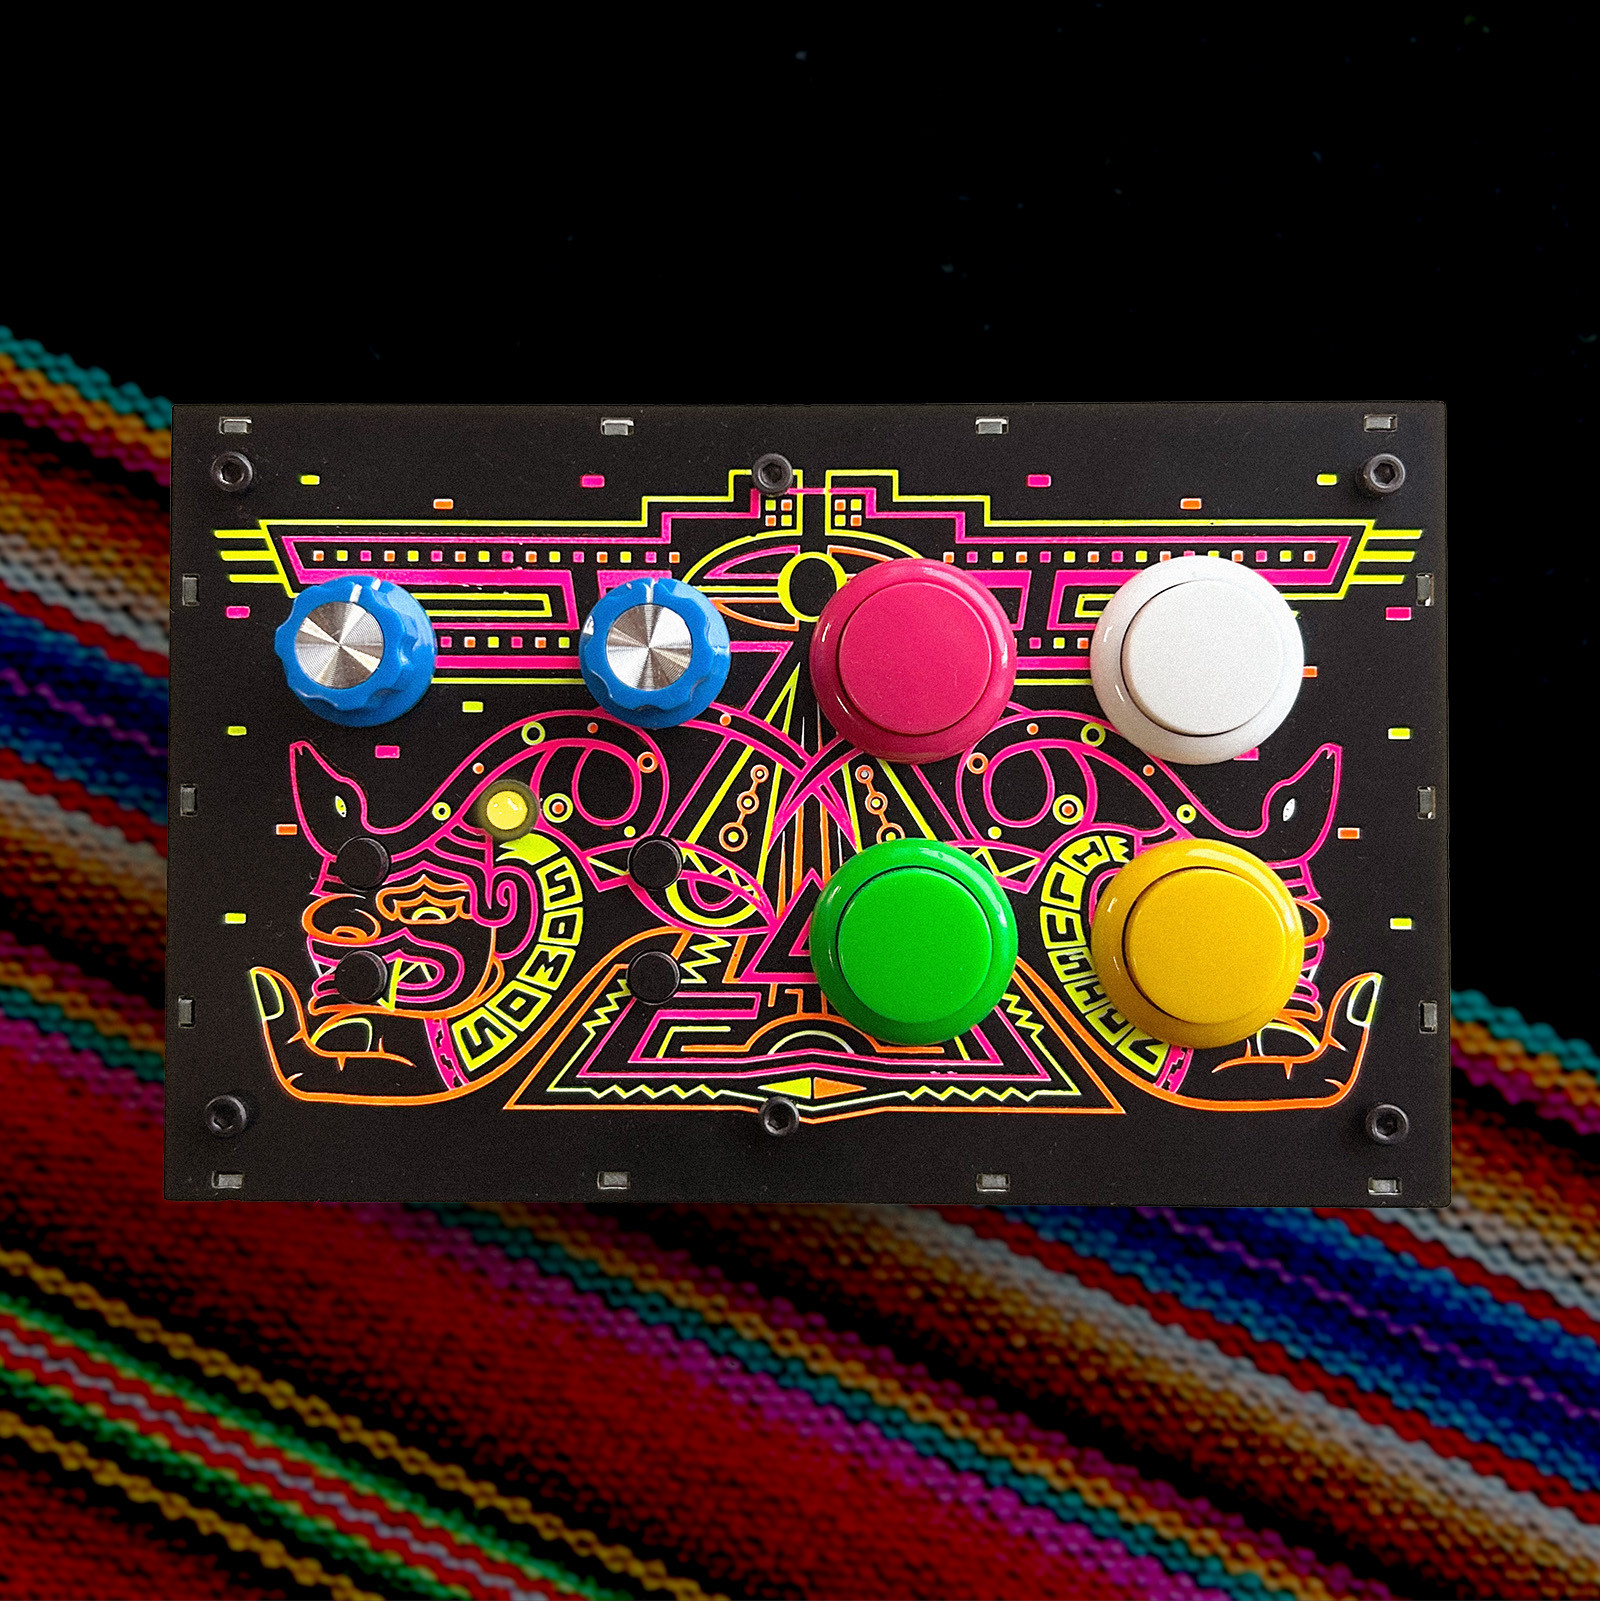
\includegraphics[width=0.6\textwidth,height=5cm,keepaspectratio]{./imagenes/referencias/oficina-de-sonido-hanan-cumbia.jpg}
    \caption[Hanan Cumbia (HTR-1), Oficina de Sonido]{Hanan Cumbia (HTR-1) de Oficina de Sonido. Fuente: \parencite{oficinadesonido_hanancumbia_sinfecha}.}
    \label{fig:oficina-de-sonido-hanancumbia}
\end{figure}

My First Modular fue financiado mediante una campaña de crowdfunding en Kickstarter \footcite{oficinadesonido_myfirstmodular_2023}, y la empresa ha explorado también nuevas estrategias de secuenciadores.

\subsubsection{Sonic Liberation Devices}

La práctica de esta cooperativa está situada en torno a la computación aplicada a la música como una forma de resistencia política, además de enlazar tanto el diseño como la manufactura de sintetizadores con su enseñanza y el compartir. Este 2026 lanzaron su primer sintetizador del tipo máquina de ritmos con énfasis en música no hegemónica.

\begin{figure}[!htbp]
    \centering
    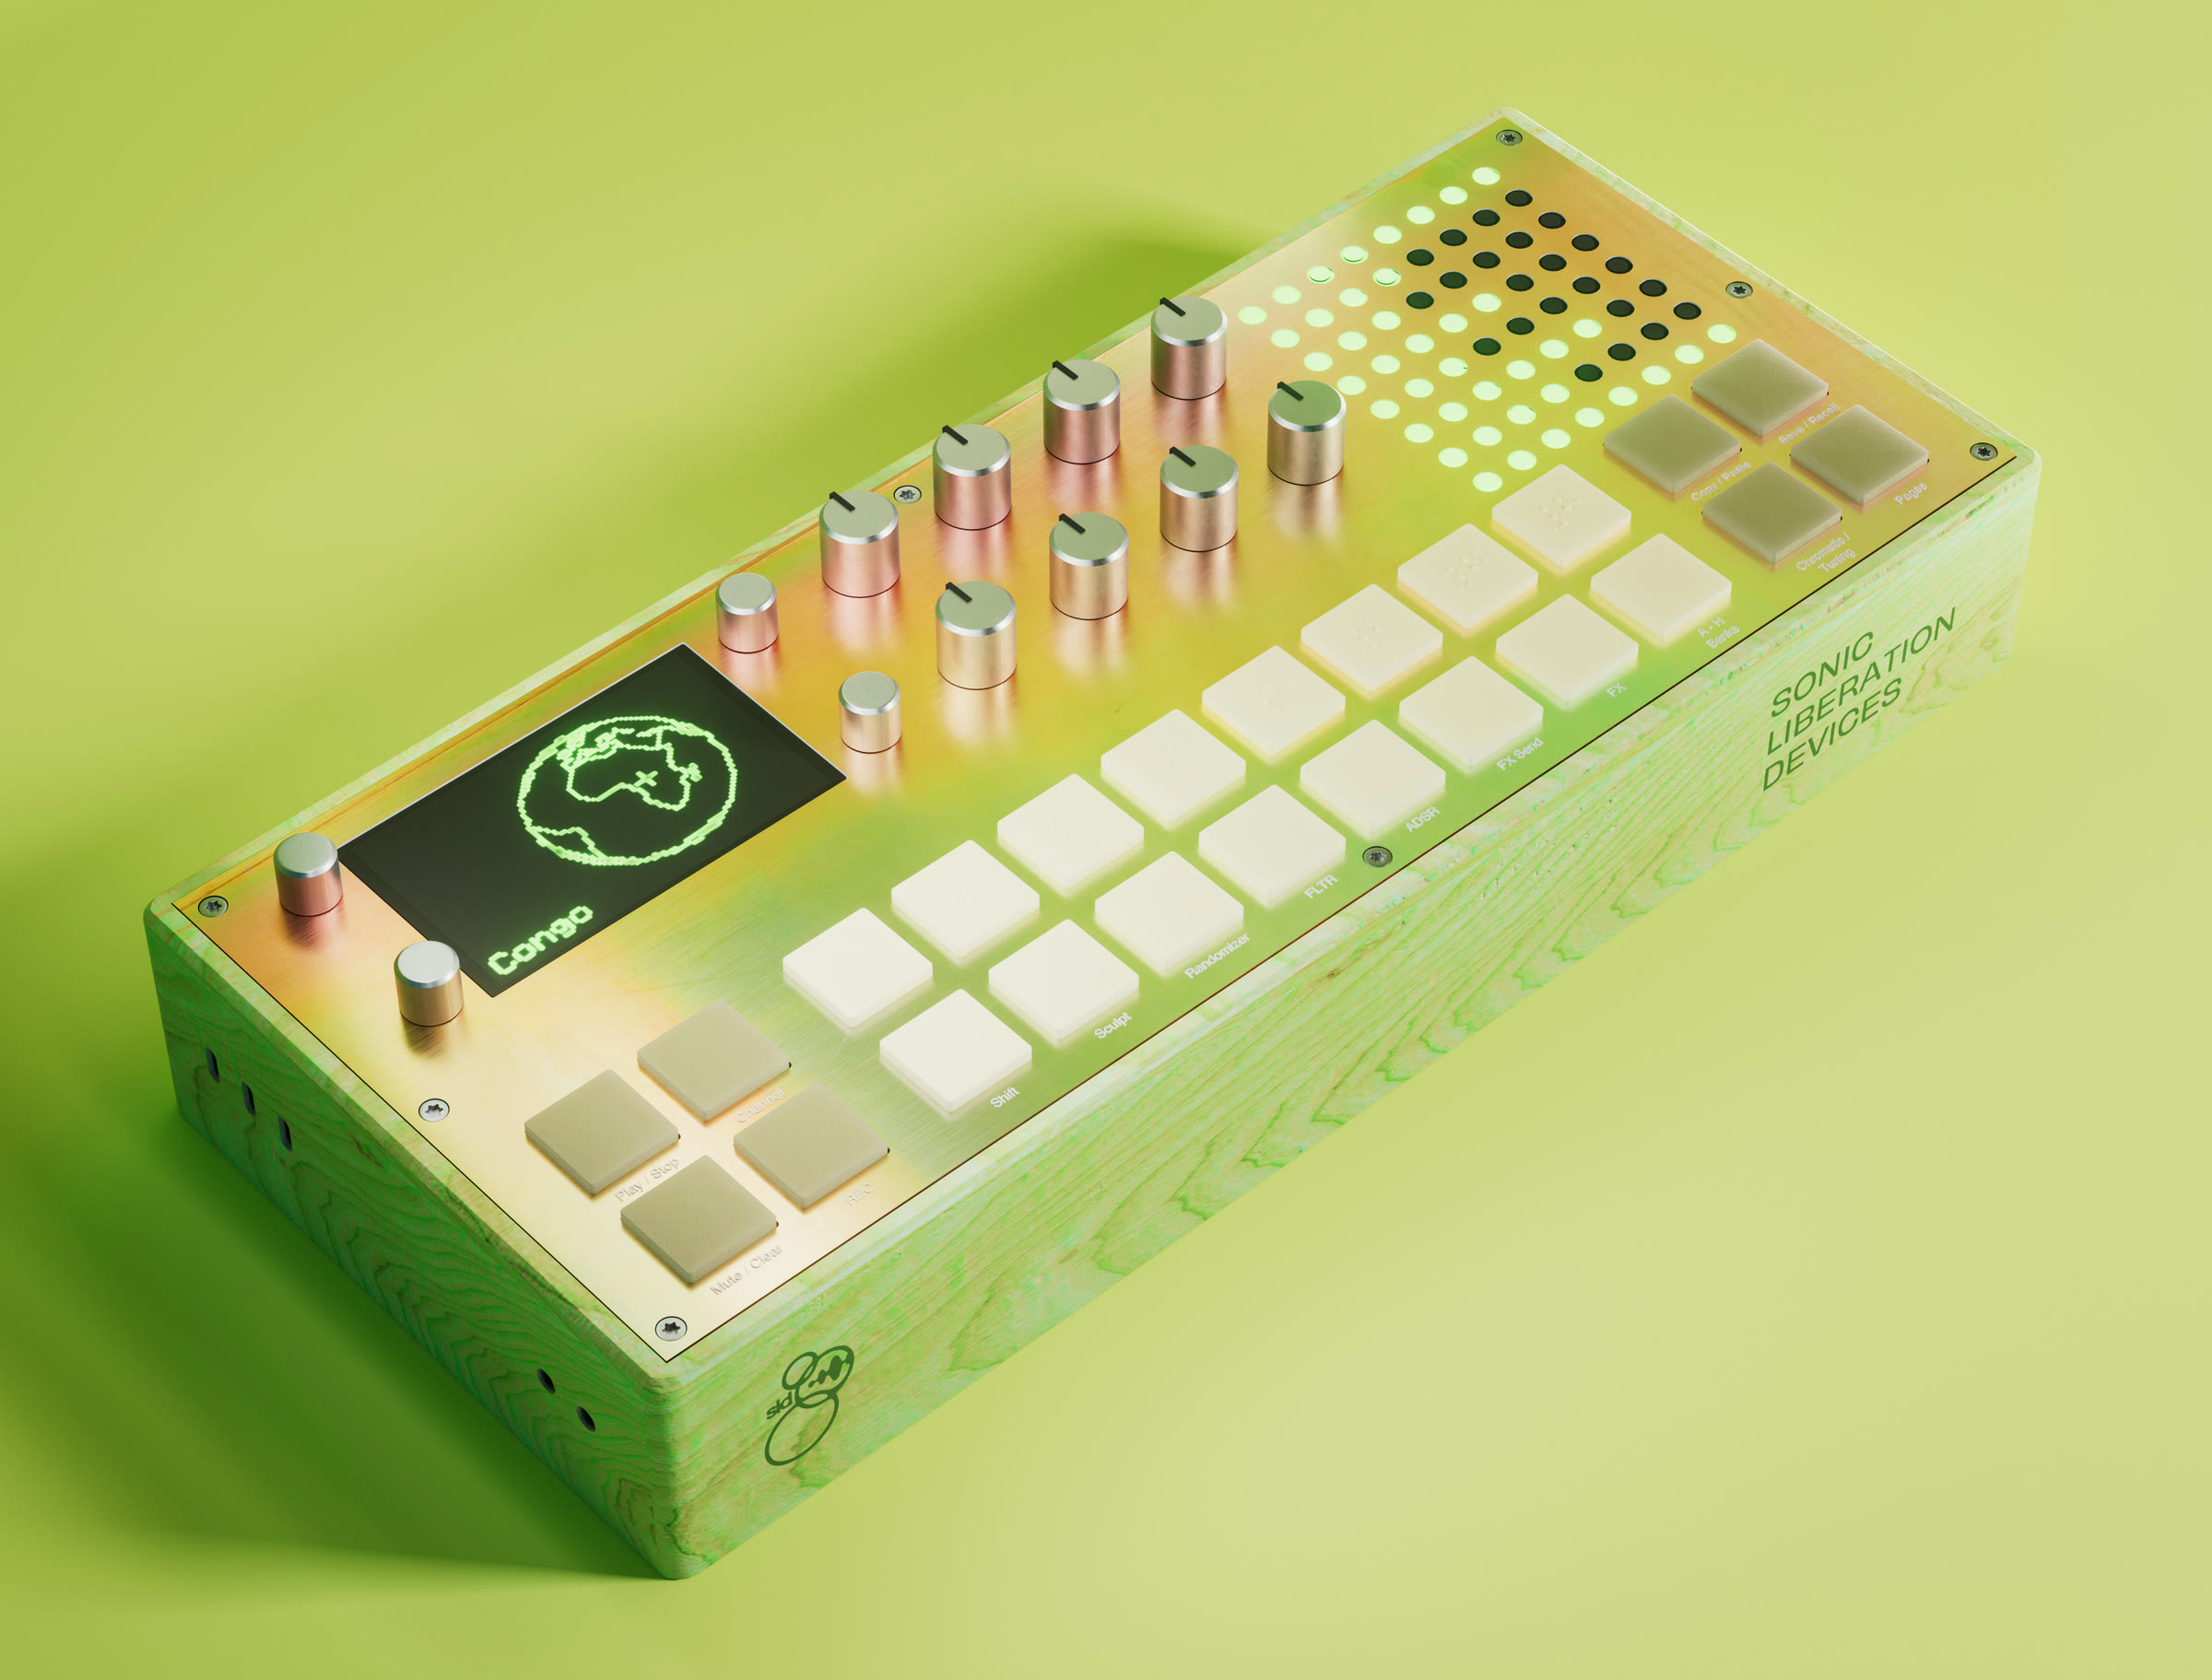
\includegraphics[width=0.6\textwidth,height=5cm,keepaspectratio]{./imagenes/referencias/sonic-liberation-devices-global-south-machine-drum-and-sampler.jpg}
    \caption[Global South Machine Drum and Sampler, Sonic Liberation Devices]{Global South Machine Drum and Sampler de Sonic Liberation Devices. Fuente: \parencite{sonic_liberation_devices_global_south_machine_drum_and_sampler_sinfecha}.}
    \label{fig:sonic-liberation-devices-global-south-machine-drum-and-sampler}
\end{figure}

\subsection{Novedad de la propuesta}

El estado del arte ha mostrado que existen muchos referentes en el mundo que pueden ser catalogados como popusintesíntesis al menos en partes de sus preceptos de filosofía, diseño y fabricación de sintetizadores sonoros.

Gran parte del corpus estudiado asume eso sí distintos tipos de conocimientos específicos para distintos públicos, agregando barreras que alejan de lo popular, por ejemplo: están en inglés \footcite{edstrom_arduino_2016} o japonés \footcite{oohashi_strange_2021} o alemán \footcite{kruse_modulare_2024}, presuponen entrenamientos formales en electrónica o computación, asumen el dominio y acceso a herramientas mecánicas y espaciales, presuponen conocimientos y práctica de arte conceptual o música.

Esta propuesta de popusintesíntesis entonces es novedosa al hacerse cargo de la dimensión metafórica y conceptual necesaria para entender las artes sonoras, de tener un enfoque que articula lo conceptual con la implementación material, sin depender de algún software o hardware en particular, y de tener como precepto la realización de herramientas paramétricas que permitan no tener un sintetizador en particular, sino que una constelación de subproductos y artefactos que permiten la emergencia de nuevas síntesis. También se incluye la dimensión de reflexión de infraestructura tanto comercial como académica que permite que esta investigación florezca, con las menores barreras de acceso posibles, y con la mayor amplitud de mente posible sobre síntesis sonora, justificándose así sus aportes.

\end{document}